\paragraph{}
Rappelons d'abord brievement ce qu'est une chaîne de Markov. Une chaîne de Markov est un outil mathématique stochastique, qui utilise un principe de "non-mémoire". Tout état d'un système est simplement calculé à partir du précédent, ce qui en facilite l'analyse.
\\\\
Ces chaînes sont simplement décrites mathématiquement comme suit avec $X_1, X_2,..., X_t$ une suite de variables aléatoires qui définit une chaîne de Markov
si (pour t > 1) elle suit cette relation :
\begin{equation*}
  \mathbb{P}(X_1, X_2, ..., X_t) = \mathbb{P}(X_1)\prod_{l = 2}^{t}\mathbb{P}(X_l | X_{l-1}) 
\end{equation*}

\subsubsection{}

Nous calculons donc pour des valeurs de $t$ croissantes les différentes valeurs demandées, ici avec $t = 20$ (suffit pour avoir convergé) :
\begin{itemize}
  \item Cas de base distribué uniformément : $\mathbb{P}(X_t = x) = 
  \begin{pmatrix}
    0.3488 & 0.0698 & 0.2326 & 0.3488\\
  \end{pmatrix}$ avec $x = 1, 2, 3, 4$
  \item Cas de base fixé : $\mathbb{P}(X_t = x) = 
  \begin{pmatrix}
    0.3488 & 0.0698 & 0.2326 & 0.3488\\
  \end{pmatrix}$ avec $x = 1, 2, 3, 4$
  \item $Q^t = 
  \begin{pmatrix}
  0.3488 & 0.0698 & 0.2326 & 0.3488\\
  0.3488 & 0.0698 & 0.2326 & 0.3488\\
  0.3488 & 0.0698 & 0.2326 & 0.3488\\
  0.3488 & 0.0698 & 0.2326 & 0.3488\\
  \end{pmatrix}$ 
\end{itemize}

On remarque donc bien une convergence vers des probabilités et ceci peut importe le cas de départ, on peut montrer cette convergence sur les figures ci-dessous :
\begin{figure}[h!]
  \centering
  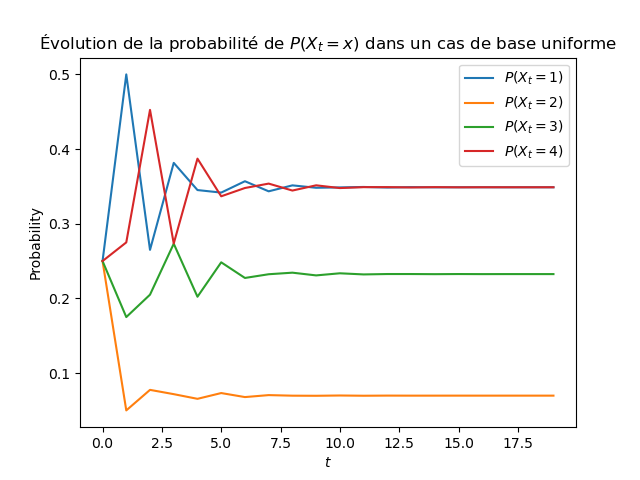
\includegraphics[width=0.5\textwidth]{figs/evo_unif.png}
  \caption{Évolution des probabilités dans une distribution de départ uniforme}
  \label{fig:unif}
\end{figure}
\\
\begin{figure}[h!]
  \centering
  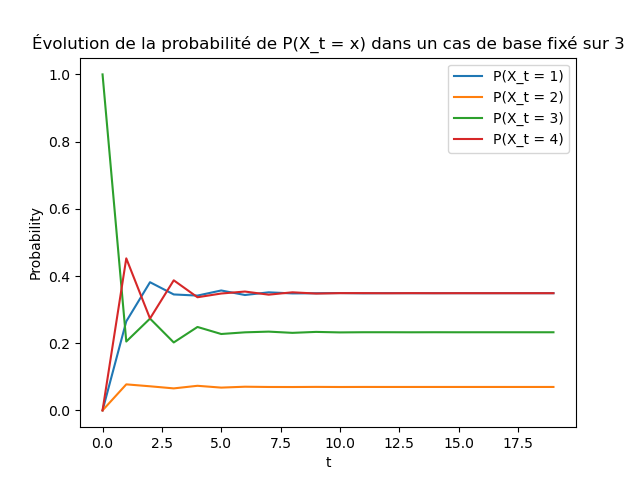
\includegraphics[width=0.5\textwidth]{figs/evo_fixed.png}
  \caption{Évolution des probabilités dans une distribution de départ fixée sur 3}
  \label{fig:fixed}
\end{figure}

On remarque qu'après une vingtaine d'itérations on obtient la relation suivante :

\begin{equation*}
  Q^t = Q^{t-1}
\end{equation*}

On en déduit donc que $\lim_{t \rightarrow \infty} Q^t \approx Q^{20} $, en effet chaque ligne de $Q^t$ est égale à $[0.3488 , 0.0698 , 0.2326 , 0.3488]$. On a déjà remarqué dans les figures \ref{fig:unif} et \ref{fig:fixed} que peut importe le 
point de départ, on converge vers les mêmes probabilités après un nombre suffisant d'itérations on montre alors avec $\pi_{t,\text{uniforme}}$ représentant la distribution des probabilités au pas de temps $t$ dans le cas d'une 
distribution de base uniforme et $\pi_{t,\text{fixé}}$ représentant la distribution des probabilités au pas de temps $t$ dans le cas d'une 
distribution de base fixée sur le cas $3$ :  

\begin{align*}
  \pi_{21,\text{uniforme}} &= \pi_{20,\text{uniforme}} Q = \pi_{20,\text{uniforme}}\\
  \pi_{21,\text{fixé}} &= \pi_{20,\text{fixé}} Q = \pi_{20,\text{fixé}} 
\end{align*}

On dit d'une distribution qu'elle est stationnaire si $\pi_t = \pi_t Q$, nous considérons donc nos deux distributions comme stationnaires et elles admettent les propriétés suivantes :\\
\begin{itemize}
  \item Ergodicité si elle est égale aux lignes de $\lim_{t \rightarrow \infty} Q^t$, comme prouvé dans la sous-section \ref{section:1.1.4}.
  \item Unicité si la châine de Markov est irréductible.
\end{itemize}

\subsubsection{}

Afin de déduire la distribution stationnaire $\pi_{\infty}$ de notre chaîne qui est décrite comme suit :
\begin{equation*}
  [\pi_\infty]_j = \lim_{t \rightarrow \infty} \mathbb{P}(X_t = j)
\end{equation*}

Nous allons simplement calculer $\mathbb{P}(X_t)$ avec un grand $t$ ce qui nous donne :
\begin{equation*}
  \pi_{\infty} = 
  \begin{pmatrix}
    0.3488 & 0.0698 & 0.2326 & 0.3488
  \end{pmatrix}
\end{equation*}
\newpage
\subsubsection{}
Afin de vérifier les résultats obtenus, nous effectuons des réalisations de notre chaîne de Markov. Nous pouvons mettre en tableau la proportion de réalisation 
de chaque état lors de tests avec un nombre de pas croissant. Nous utilisons un point de départ distribué uniformément entre les 4 états car il a été prouvé
plus haut que ça n'avait pas d'influence.

\begin{table}[h!]
  \begin{tabular}{|c|c|c|c|c|}
  \hline
  \# Pas / État & \multicolumn{1}{c|}{1} & \multicolumn{1}{c|}{2} & \multicolumn{1}{c|}{3} & 4 \\ \hline
  100     & 0.35    & 0.05   & 0.21    & 0.39    \\ \hline
  1000    & 0.351   & 0.075  & 0.23    & 0.344   \\ \hline
  10000   & 0.346   & 0.064  & 0.236   & 0.354   \\ \hline
  100000  & 0.3501  & 0.0722 & 0.228   & 0.3497  \\ \hline
  1000000 & 0.34902 & 0.6757 & 0.23422 & 0.34919 \\ \hline
  \end{tabular}
  \centering
  \caption{Proportion des états obtenus en fonction de nombre de pas}
  \label{tab:table-prop}
\end{table}
En comparant ce tableau avec les résultats obtenus avec les valeurs précédement obtenus, on remarque bien que les proportions sont respectées et font sens, on converge bien 
vers les mêmes valeurs.
\\\\
Pour montrer plus de détails, on montre qu'on approche bien des valeurs des lignes de $\lim_{t \rightarrow \infty} Q^t$ avec des fluctuations qui s'atténuent plus $t$ augmente :

\begin{figure}[ht] 
  \begin{minipage}[b]{0.5\linewidth}
    \centering
    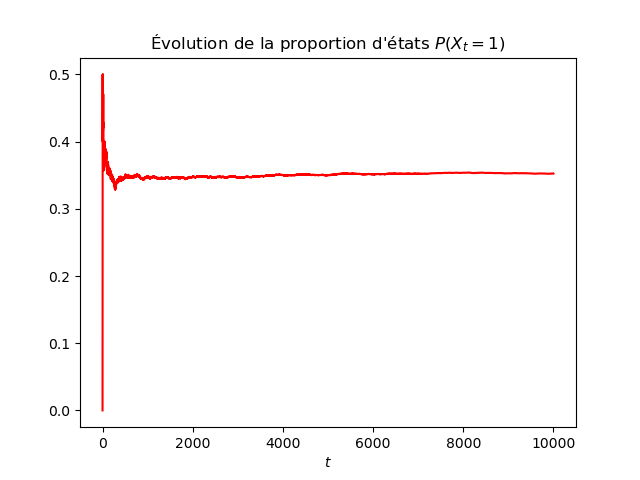
\includegraphics[width=.5\linewidth]{figs/evo1.png} 
    \caption{Proportion de l'état 1} 
    \vspace{4ex}
  \end{minipage}%%
  \begin{minipage}[b]{0.5\linewidth}
    \centering
    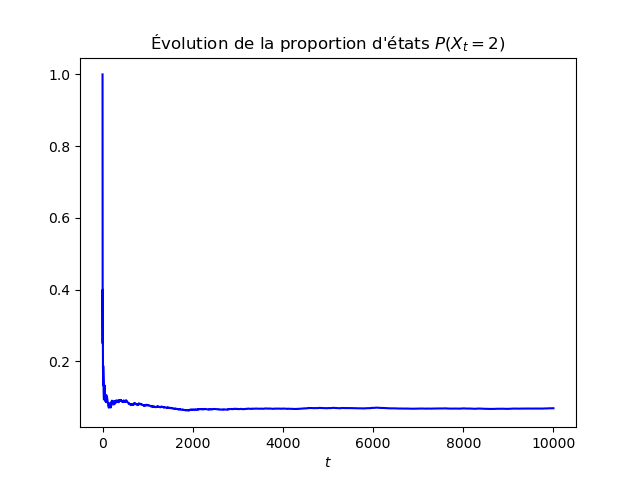
\includegraphics[width=.5\linewidth]{figs/evo2.png} 
    \caption{Proportion de l'état 2} 
    \vspace{4ex}
  \end{minipage} 
  \begin{minipage}[b]{0.5\linewidth}
    \centering
    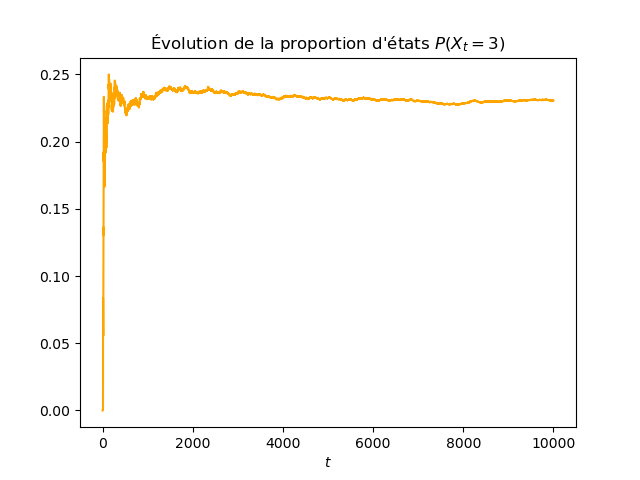
\includegraphics[width=.5\linewidth]{figs/evo3.png} 
    \caption{Proportion de l'état 3} 
    \vspace{4ex}
  \end{minipage}
  \begin{minipage}[b]{0.5\linewidth}
    \centering
    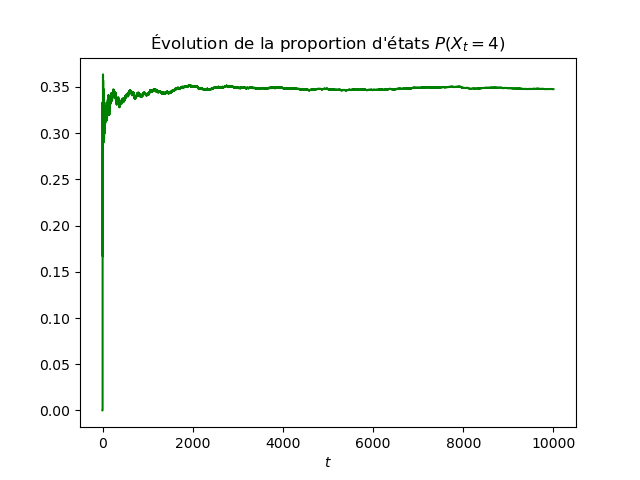
\includegraphics[width=.5\linewidth]{figs/evo4.png} 
    \caption{Proportion de l'état 4} 
    \vspace{4ex}
  \end{minipage} 
\end{figure}

\subsubsection{}
\label{section:1.1.4}
Après ces premières expériences sur les chaînes de Markov et après avoir remarqué que les distributions sont comme attendu stationnaires, nous pouvons conclure que la chaîne de Markov que nous avons réalisé est ergodique.
Une telle chaîne permet d'obtenir la distribution stationnaire de deux manières différentes, soit en effectuant des réalisations différentes, soit en effectuant une chaîne assez longue.
\\\\
Pour être ergodique, une chaîne doit respecter 3 conditions : avoir un espace finit, être irréductible et être apériodique. Analysons ces 3 conditions dans notre cas précis.

\begin{itemize}
  \item Nous avons bien un espace finit d'états (1,2,3,4).
  \item Nous avons bien une chaîne irréductible car la probabilité d'accéder à chaque noeud depuis un autre noeud est non nulle. On peut remarquer cela en observant bien que les noeuds apparaissent plusieurs fois lors de nos réalisations de la chaîne de Markov. On ne reste pas bloqués dans un sous-espace d'états.
  \item Nous avons bien une chaîne de Markov apériodique car quand on calcule 
  \begin{equation*}
    Q = \begin{pmatrix}
      0 & 0.1 & 0.1 & 0.8\\
      1 & 0 & 0 & 0\\
      0.6 & 0 & 0.1 & 0.3\\
      0.4 & 0.1 0.5 & 0
    \end{pmatrix}
    Q^2 = \begin{pmatrix}
      0.48 & 0.08 & 0.41 & 0.03\\
      0 & 0.\\
      \\
    \end{pmatrix}
  \end{equation*}

  \begin{equation*}
    Q^3 = \begin{pmatrix}
      0.338 & 0.051 & 0.104 & 0.507\\
      0.48 & 0.08 & 0.41 & 0.03\\
      0.426 & 0.069 & 0.295 & 0.21\\
      0.282 & 0.087 & 0.284 & 0.347
    \end{pmatrix}
\end{equation*}
,on remarque bien que 
\end{itemize}